\documentclass[11pt,a4paper]{article}

\usepackage{graphicx}
\usepackage{amsmath}
%\usepackage{DHUcs}
%\usepackage[nonfrench, finemath]{kotex}
%\usepackage[hangul,nonfrench,finemath]{kotex}
%\usepackage[default]{dhucs-interword}
%\usehangulfontspec{ut}
%\usepackage[hangul]{dhucs-setspace}
%\usepackage{dhucs-gremph}
\usepackage{dhucs}

\usepackage{ifpdf}
\ifpdf
  \usepackage[unicode,pdftex,colorlinks]{hyperref}
  \input glyphtounicode\pdfgentounicode=1
\else
  \usepackage[unicode,dvipdfm,colorlinks]{hyperref}
\fi


\usepackage{graphicx}
\usepackage{subfig}
%\usepackage{multirow}
%\usepackage{setspace}
%\usepackage{cite}
%\usepackage{apacite}


\newcommand{\boldHeader}[1]{\vspace{1.5ex}\noindent\textbf{#1}:}

\title{Iguana simulation}

\begin{document}
\begin{center}
{\LARGE \textbf{Iguana simulation}}
\vspace{0.3cm}


\today
\end{center}


\section{Motivation}

사람이나 이구아나 등 동물의 움직임을 가상환경에서 재현하기 위한 simulation방법으로 기존에는 rigid-body simulation 이 일반적으로 사용되었다. 하지만 이러한 방법은 동물의 근육, 지방, 연골 등 연조직의 세밀한 움직임을 재현하기 어렵다는 문제점이 있다. 본 연구에서는 flexible-body simulation 기법인 mass-spring simulation을 사용하여 이러한 문제점을 개선하고자 한다. 또한 Flexible body simulation기법을 사용하더라도, 재질 특성을 조정함으로써 rigid body simulation을 근사하는 것이 가능하지만, 그 역은 쉽지 않다는 점에서 flexible body simulation은 가상 캐릭터의 표현력을 넓히는 의미를 가진다.
\begin{figure}[h]
\center

\subfloat[]{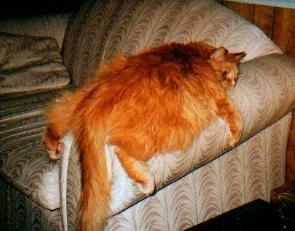
\includegraphics[height=4cm]{figures/cat.jpg}}~
\subfloat[]{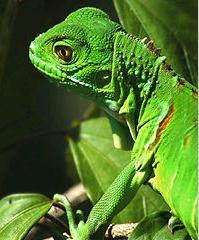
\includegraphics[height=4cm]{figures/iguana.jpg}}~
\subfloat[]{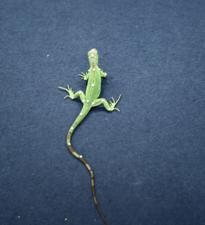
\includegraphics[height=4cm]{figures/marker.jpg}}
\caption{\label{figure1}}
\end{figure}

\section{Overview}
\subsection{동작 포착.}
               
이구아나에 총 22개의 마커를 부착하고 (각 다리에 3~4개, 몸통에 8개) 일반적인 광학식 모션캡쳐 장비를 사용하여 이구아나의 동작을 포착하였다 (See Figure~\ref{figure1} (c)). Marker 위치 정보는 IK를 사용하여 관절각 정보로 변환하였다. 모든 관절각을 정확하게 추출하기에 충분한 개수의 마커를 이구아나 subject에 부착하는 것이 불가능했기 때문에, IK를 푸는 과정에서 관절각에 제한범위를 두고, 필요에 따라 DOF를 제한하여 유일해를 가지도록 보장하였다.
\begin{figure}[h]
\center
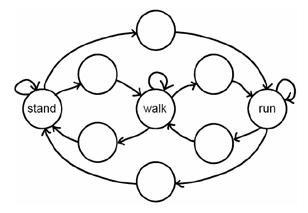
\includegraphics[height=5cm]{figures/graph.jpg}
\caption{동작 전이 그래프\label{graph}}
\end{figure}

\subsection{Kinematic controller}
이구아나 보행동작의 제어를 위하여 포착된 데이타를 가지고 [Kwon and Shin 2005]에서 사용된 것과 유사한 동작그래프를 만들었다. (Figure \ref{graph})
그래프의 각 노드는 걷기나 뛰기 동작, 또는 걷기와 뛰기 사이의 전이 동작들을 여러개 가지고 있고, 각 세그먼트는 보행동작 반주기에 해당하는 길이를 가지고 있다. 즉 왼쪽 앞발을 내딛기 시작하는 동작 세그먼트는 오른쪽 앞발을 내딛기 시작하는 순간 끝이난다. 이구아나의 동작은 평지에서만 촬영하였지만, 다양한 형태의 지형에서 걷는 동작을 생성하기 위해 동작 변형 기능이 요구된다. 간단하게 평지에서 생성된 동작의 각 프레임을 독립적으로 ik를 이용하여 지형위에 맞추는 경우, 이구아나가 지형의 변화에 미리 대응하지 못하고 갑작스럽게 다리를 들어올리거나 떨어트리는 동작을 생성하게 된다. 대신 우리는 약간의 look-ahead(1/4초)를 사용하여, 1/4초 후의 자세와 위치를 예측하여 그 시간에 각 다리가 지면 아래에 있지 않도록 ik를 수행하였고, displacement map을 사용하여 관절각 변화가 시간에 따라 부드럽게 변화하도록 보장하였다. 매 프레임 displacement map을 update하여, 예측 못한 상황의 변화에도 대응할 수 있도록 하였다. IK를 수행하기 전과 후의 자세 변화가 큰 경우, IK를 수행하는 것 만으로 동작이 이상하게 변할 수 있다. 이를 막기 위하여 두 단계로 IK를 수행하였다. 첫번째 단계에서는 rigid transform만 사용하여 각 다리의 지면에서의 높이가 예제 동작에서의 높이와 최대한 유사해지도록 근사적으로 자세를 지면위에 올려 놓는다. 이는 전형적인 shape matching문제로써 우리는 [Horn1987] 방법을 사용하였다. 첫 번째 단계의 수행후에도 다리 또는 꼬리가 지면 아래에 있는 경우, 추가적인 IK를 통해 꺼내주었다.
\subsection{Dynamic controller}
Kinematic controller만을 사용하여 생성한 동작은 물리적 타당성이 고려되지 않았기 때문에, 사실성이 떨어지고, 외부 충격에 반응동작을 생성하기 어렵다는 문제점이 있다. dynamic controller는 mass-spring simulation을 통해 kinematic controller가 생성한 동작을 사실적으로 따라가는 가상 캐릭터를 생성한다. 먼저 우리는 관절각 정보를 이용해 그림 ~\ref{target}에 보이는 target mesh의 애니메이션을 생성한다. 이를 위해 dual quaternion 을 이용한 skinning기법을 사용하였다. [Kavan et al. 2008]
                             
\begin{figure}[h]
\center
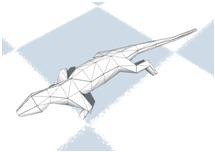
\includegraphics[height=5cm]{figures/target.jpg}
\caption{Target mesh\label{target}}
\end{figure}

                                 
위 메쉬의 정점을 mass point로 사용하고, 메시 상에서 거리가 특정 threshhold보다 가까운 두 정점 사이에 spring을 삽입하여 그림 \ref{model}과 같은 매스 스프링 모델을 구성하였다. 각 mass point의 질량은 인접한 삼각형의 면적에 비례하도록 설정하였다.
          

\begin{figure}[h]
\center
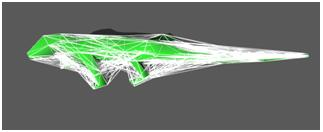
\includegraphics[height=5cm]{figures/model.jpg}
\caption{Mass-spring model\label{model}}
\end{figure}
		  
                      
Flexible body simulation에 사용되는 다양한 기법 중 mass-spring기법을 선택한 이유는, [baraff98] 등 imclicit구현을 사용하면 실시간에 robust한 시뮬레이션이 가능하고, 스프링에 힘을 가하거나 길이를 조정하는 방식으로 직관적인 제어가 가능했기 때문이다. 일반적인 rigid-body simulation과 비교해서는 무릎 관절의 singularity문제가 없으므로 knee-popping이나 robot-like walking 등 로보틱스 분야의 알려진 어려움을 피해갈 수 있고, 재질 특성을 조절함으로써 rigid한 부분과 non-rigid한 부분의 simulation을 동일한 방식으로 시뮬레이션 할 수 있다는 장점을 가진다.
그림 3에 도시된 모델이 target mesh의 움직임을 따라가도록 하기 위해서는, 간단하게 각 스프링의 rest-length를 target mesh의 해당 정점 사이의 거리로 세팅하는 방법을 사용할 수 있다. 실험결과 이 간단한 방법으로도 이구아나가 평지에서 문제없이 걷는 등 가능성이 보였지만, 발과 배를 땅에 끌면서 걷는 등 부자연스러운 부분이 발견 되었다. 이 문제를 해결하기 위하여 우리는 제어 신호를 최적화해서 타겟 메쉬를 물리 모델이 최대한 따라가도록 하는 접근법을 취한다.
Let $\mathbf x_i$ and $\mathbf x'_i(\mathbf r_i)$ be the vertex positions of the target mesh and simulated mesh at frame i, respectively. 
여기서 simulated mesh의 정점 위치 $\mathbf x'_i$ 는 i번째 프레임의 모든 스프링의 rest length의 집합 $\mathbf r_i$의 함수이다. 
어떤 동작 세그먼트에 대해서 target mesh와 simulation mesh의 차이를 최소화하기 위해서는 이상적으로는 아래와 같은 최적화를 수행해야한다.
\begin{equation}
\left\{ \mathbf{r}_{i}\right\} _{i\in[s,e]}=\arg\min\sum_{s}^{e}\left\Vert\mathbf{x}_{i}-\mathbf{x}'_{i}\left(\mathbf{r}_{i}\right)\right\Vert^{2}.
\end{equation}
하지만, 이 방법은 $\mathbf{r}_{i}$의 차원이 아주 높고, 위 목적함수 값을 단 한번 계산하기 위해서도 시뮬레이션을 한번 수행해야해서 시간이 많이 걸리는 이유로 현실적으로 사용이 불가능하다. 그 대신 우리는 위 목적함수를 아래와 같이 변경하여 문제를 푸는 방법을 제안한다.
\begin{equation}
\left\{ \mathbf{r}_{i}\right\} _{i\in[s,e]}=\arg\min\sum_{s}^{e}\left\Vert\mathbf{l}_{i}-\mathbf{l}'_{i}\left(\mathbf{r}_{i}\right)\right\Vert^{2}.
\end{equation}
여기서 $\mathbf l_i$ and $\mathbf l'_i(\mathbf r_i)$ 는 스프링으로 연결된 두 정점사이의 실제 길이들을 target mesh와 simulated mesh에서 각각 계산한 값을 의미한다. 그러면 feed-back error learning 기법과 유사한 방식으로 스프링 길이의 error $mathbf e_i = mathbf{l}_{i}-\mathbf{l}'_{i}\left(\mathbf{r}_{i}\right)$에 비례하게 rest length $\mathbf{r}_{i}$를 조정해주는 방법을 사용할 수 있다. 

$\mathbf r_i$ 을 $\mathbf l_i+\mathbf o_i$ 라고 정의하자. 여기서 $\mathbf l_i$는 상수 이므로 우리는 $\mathbf r_i$ 대신 offset $\mathbf o_i$를 최적화하는 문제로 바꿀 수 있다. 제안된 최적화 방법은 우선 $\mathbf o_i$를 0으로 초기화하고, 매 iteration마다 offset $\mathbf o_i$를 아래 식을 사용해서 update한다.
\begin{equation}
\mathbf o_i \leftarrow \mathbf o_i + \alpha\mathbf e_i.
\end{equation}
여기서 learning rate $\alpha$는 0.05정도가 실험적으로 잘 동작했다. 위 update는 모든 프레임과 모든 스프링에 대해서 동시에 이루어진다. 이때 learning rate를 모든 스프링에 대해서 동일하게 사용하는 것보다는 스프링의 중요도에 따라 다르게 사용하는 것이 더 좋은 최적화 값을 얻게 할 것임은 자명하다. 우리는 randomized search방법을 사용하여 매 이터레이션마다 10$\%$정도의 스프링만 random하게 선택하여 이들에만 learning rate에 non-zero 값을 assign한 learning rate set을 20개 정도 만들어, 이 중 가장 SSE = $\sum_s^e\left\Vert\mathbf e^i\right\Vert^2$를 최소화하는 set을 선택해 update를 진행한다. 모든 set이 SSE를 증가시키는 경우 learning rate를 10\%감소시켜서 다시 시도 하고, learning rate가 특정 threshold보다 작아지면 iteration을 중지한다.

\subsection{Mesh deformation}
시뮬

\section{Results}

최적화 과정을 거치기전의 SSE 가 33024 인 dataset에 대해서, randomized 최적화 수행후 SSE는 14017이었다. Randomized 과정을 적용하지 않은 최적화의 경우 SSE=22017에서 종료되었다.



\section{Limitations }
The object function is coordinate invariant. 
\section{Future work}
\begin{itemize}
\item {Low stiffness (impulse demo.) }
\item{Use high quality mesh}
\item {Two-level optimization }
\subitem{Skeleton-level optimization using equation 1}
\subitem{Spring-level optimization using equation 2 }
\end{itemize}


%Target mesh should be updated properly to drive simulated mesh 
%	Position correction 
%	Orientation correction 
%	Vertical orientation difference 
%	Footstep correction 

\section*{References}

[HORN 1987] HORN, B. K. P. 1987. Closed-form solution of absolute orientation using unit quaternions. Journal of the Optical Society of America A 4, 4, 629~642.


\end{document}
